%==============================================================================
\chapter{In silico identification of calcium dynamics and sarcomere targets for recovering left ventricular function in rat heart failure with preserved ejection fraction}\label{cha:chapter7}
%==============================================================================
%
%
%
\begin{remark}{Outline}
    In this chapter, we build an emulator that can map both calcium, sarcomere, tissue and hemodynamics properties to the LV function, using the personalised SHAM rat heart contraction model as simulator. After having characterised the model outputs' sensitivities to model inputs, starting from the healthy reference rat model we create a model of the $20$-week old obese ZSF1 rat, a well-enstablished animal model of heart failure with preserved ejection fraction. We then use different sub-groups of input parameters as targets of a re-fitting, history matching procedure, with the aim of recoverying the ZSF1 rat model back to the healthy state. The selected groups of parameters mimick the action of possible calcium-, thin filament-, thick filament-, whole sarcomere-targeting compounds. The implemented framework shows that it is possible to \textit{in silico} efficiently identify possible pharmacological interventions on the sarcomere to treat HFpEF in rats.
\end{remark}


%
%
%
\section{Motivation}\label{sec:ch7motivation}
\todo{this is Abstract copy-pasted from the paper: adapt it to thesis}

\noindent
Heart failure with preserved ejection fraction (HFpEF) is a complex disease associated with multiple co-morbidities, where impaired cardiac mechanics are often the end effect. At the cellular level, cardiac mechanics can be pharmacologically manipulated by altering calcium signalling and the sarcomere. However, the link between cellular level modulations and whole organ pump function is incompletely understood. Our goal is to develop and use a multi-scale computational cardiac mechanics models of the obese ZSF1 rat HFpEF to identify important biomechanical mechanisms that underpin impaired cardiac function and to predict how whole-heart mechanical function can be recovered through altering cellular calcium dynamics and/or cellular contraction. The rat heart was modelled using a $3$D biventricular biomechanics model. Biomechanics were described by $16$ parameters, corresponding to intracellular calcium transient, sarcomere dynamics, cardiac tissue and hemodynamics properties. The model simulated left ventricular (LV) pressure-volume loops that were described by $14$ scalar features. We trained a Gaussian process emulator (GPE) to map the $16$ input parameters to each of the $14$ outputs. A global sensitivity analysis identified calcium dynamics and thin and thick filament kinetics as key determinants of the organ scale pump function. We employed Bayesian history matching to build a model of the ZSF1 rat heart. Next, we recovered the LV function, described by ejection fraction, peak pressure, maximum rate of pressure rise and isovolumetric relaxation time constant. We found that by manipulating calcium, thin and thick filament properties we can recover $\SI{34}{\percent}$, $\SI{28}{\percent}$ and $\SI{24}{\percent}$ of the LV function in the ZSF1 rat heart, respectively, and $\SI{39}{\percent}$ if we manipulate all of them together. We demonstrated how a combination of biophysically based models and their derived emulators can be used to identify potential pharmacological targets. We predicted that cardiac function can be best recovered in ZSF1 rats by desensitising the myofilament and reducing the affinity to intracellular calcium concentration and overall prolonging permanence in active force generating state.

\vspace{0.2cm}\noindent
\todo{this is AuthorSummary copy-pasted from the paper: adapt it to thesis}

\noindent
We developed a computational model of the ZSF1 rat model of heart failure with preserved ejection fraction. We validated that the model can link simulated pharmacological interventions from cellular to whole heart pump function. Our computational model identified calcium dynamics as the main determinant of left ventricular contractile behaviour. We demonstrated that the highest degree of LV function recovery could be achieved when calcium dynamics is manipulated in conjunction with both thin and thick filament kinetics.

\vspace{0.2cm}\noindent
\todo{this is Introduction copy-pasted from the paper: adapt it to thesis}

\noindent
Heart failure (HF) is a progressive and prevalent disease. Approximately $\SI{50}{\percent}$ of patients have heart failure with preserved ejection fraction (HFpEF), characterised by impaired myocardial relaxation and often secondary to hypertension and obesity. There are limited evidence-based pharmacotherapies for HFpEF and thus HFpEF represents an unmet clinical need. Patients currently receive either angiotensin-converting enzyme inhibitors/aldosterone receptor blockers, calcium channel blockers or beta-blockers, but the mortality and the morbidity associated with the disease have so far remained high~\cite{Adamczak:2020}.

Animal models constitute a valuable research tools to investigate HFpEF, as comorbidities and other confounding factors can be more precisely controlled than in the clinical setting. However, there are no perfect animal models for HFpEF, and this is in part because it is difficult to fulfil all the features observed in human disease at the same time in animals. The currently available animal models of HFpEF have attempted to reproduce the dominant factors typically documented to cause diastolic dysfunction and HFpEF. They fall across the following macro-categories: aortic banding and systemic hypertension, diabetes mellitus and obesity, cardiometabolic syndrome and ageing. All of these animal models have been successfully established in rodents~\cite{Conceicao:2016}. Regardless of the animal model used in the process of drug discovery and development at preclinical stages, identifying pharmacological interventions that recover physiological function in the HFpEF diseased animal still remains a challenge.

In this study we aim to predict changes in myocyte function that recovers whole heart function. First, we propose a multi-scale mathematical model that maps ion channel and sarcomere function through to whole organ pump function in a HFpEF rat heart. Specifically, we want to build an \textit{in silico} representation of the \textit{$20$-week old obese ZSF1 rat}, a recently proposed HFpEF animal model. This model can then be used to identify cellular function that can be manipulated to recovered whole heart function. We propose to use this animal model to inform the selection of cellular pharmacological targets by simulating and testing their different mechanisms of action. The $20$-week old obese ZSF1 rat presents many features of a cardiometabolic syndrome such as hypertension, obesity, type $2$ mellitus, insulin resistance and HF, developing a diastolic dysfunction in parallel with left ventricular (LV) hypertrophy and left atrial (LA) dilation. As this animal model also presents exercise intolerance, an important feature diagnosed in humans, it currently constitutes a well-established~\cite{Conceicao:2016} animal model of HFpEF. From now on, we will refer to the ``$20$-weeks old obese ZSF1 rat" as the ``ZSF1 rat" for brevity.


%
%
%
\section{Methods}\label{sec:ch7methods}


%
%
%
\subsection{Rat heart contraction model}\label{sec:ratmodel}
We modelled the healthy rat heart using the personalised SHAM rat heart contraction model derived in Section~\ref{sec:ch4fittedmodels}. This rat model will be referred to as ``SHAM" throughout the next sections. Again, this model (or simulator) can be seen as a multi-scale map from input parameters to output features.

\vspace{0.2cm}
We augmented the list of parameters used previously (Sections~\ref{sec:ch4ratheartcontractionmodel}--\ref{sec:ch5ratheartcontractionmodel}) in order to have a more comprehesive description of both the calcium dynamics, sarcomere kinetics, tissue and hemodynamic boundary conditions' properties, by considering a total of $16$ parameters. Specifically, $4$ parameters encoded the shape of the calcium transient (Section~\ref{sec:ch6encodingcalciumtransientvariations}), $8$ parameters described the sarcomere dynamics ($4$ parameters were thin filament-related and $4$ were thick filament-related), and $4$ parameters described boundary conditions and tissue properties. The full list of parameters considered is reported in Table~\ref{tab:paramswithdeffinal}.

\begin{table}[!ht]
    \myfloatalign
    \begin{tabularx}{\textwidth}{llX}
    \toprule
    \tableheadline{Parameter} & \tableheadline{Units}                   & \tableheadline{Definition} \\
    \midrule
    $\dca$                    & $\SI{}{\micro\Molar}$                   & diastolic $\Ca$ concentration \\
    $\ampl$                   & $\SI{}{\micro\Molar}$                   & $\Ca$ concentration signal amplitude \\
    $\tp$                     & $\SI{}{\milli\second}$                  & time to peak $\Ca$ concentration \\
    $\rtf$                    & $\SI{}{\milli\second}$                  & time to half-maximal relaxation from peak $\Ca$ concentration \\
    $\Caif$                   & $\SI{}{\micro\Molar}$ & reference $\Ca$ thin filament sensitivity \\
    $\betaone$                & $-$                                     & phenomenological tension length-dependence scaling factor \\
    $\koff$                   & $\SI{}{\per\milli\second}$              & unbinding rate of $\Ca$ from TnC \\
    $\ntrpn$                  & $-$                                     & $\Ca$-TnC binding degree of cooperativity \\
    $\kxb$                    & $\SI{}{\per\milli\second}$              & cross-bridges cycling rate \\
    $\nxb$                    & $-$                                     & cross-bridge formation degree of cooperativity \\
    $\trpnf$                  & $-$                                     & fraction of $\Ca$-TnC bounds for half-maximal cross-bridges activation \\
    $\tref$                   & $\SI{}{\kilo\pascal}$                   & maximal reference tension \\
    $\p$                      & $\SI{}{\kilo\pascal}$                   & end-diastolic pressure \\
    $\pao$                    & $\SI{}{\kilo\pascal}$                   & aortic systolic pressure \\
    $\Z$                      & $\SI{}{\mmHg\second\per\milli\liter}$   & aortic characteristic impedance \\
    $\Cone$                   & $\SI{}{kPa}$                            & tissue stiffness \\
    \bottomrule
    \end{tabularx}
    \caption{Model parameters and their definitions.}
    \label{tab:paramswithdeffinal}
\end{table}

\vspace{0.2cm}
As for the simulator output, we described the LV function using the same $12$ scalar features used in the previous analysis (Table~\ref{tab:lvfeatures}) with the addition of other $2$ features. The full set of $14$ LV features considered is reported in Table~\ref{tab:lvfeaturesfinal}.

\begin{table}[!ht]
    \myfloatalign
    \begin{tabularx}{\textwidth}{llX}
    \toprule
    \tableheadline{LV feature}                  & \tableheadline{Units}                         & \tableheadline{Definition} \\ \midrule
    $\textrm{EDV}$                  & $\SI{}{\micro\liter}$                  & end-diastolic volume \\         
    $\textrm{ESV}$                  & $\SI{}{\micro\liter}$                  & end-systolic volume \\
    $\textrm{SV}$                   & $\SI{}{\micro\liter}$                  &  stroke volume \\
    $\textrm{EF}$                   & $\SI{}{\percent}$                      & ejection fraction \\              
    $\textrm{IVCT}$                 & $\SI{}{\milli\second}$                 & isovolumetric contraction time \\
    $\textrm{ET}$                   & $\SI{}{\milli\second}$                 & systolic ejection time \\                  
    $\textrm{IVRT}$                 & $\SI{}{\milli\second}$                 & isovolumetric relaxation time \\
    $\textrm{Tdiast}$               & $\SI{}{\milli\second}$                 & diastolic filling time \\
    $\textrm{PeakP}$                & $\SI{}{\kilo\pascal}$                  & peak systolic pressure \\
    $\textrm{Tpeak}$                & $\SI{}{\milli\second}$                 & time to peak systolic pressure \\
    $\textrm{ESP}$                  & $\SI{}{\kilo\pascal}$                  & end-systolic pressure \\
    $\textrm{maxdP}$ & $\SI{}{\kilo\pascal\per\milli\second}$ & maximum pressure rise rate \\
    $\textrm{mindP}$ & $\SI{}{\kilo\pascal\per\milli\second}$ & maximum pressure decay rate \\
    $\textrm{Tau}$   & $\SI{}{\milli\second}$ & isovolumetric pressure relaxation time constant \\
    \bottomrule
    \end{tabularx}
    \caption{Indexes of LV systolic and diastolic functions.}
    \label{tab:lvfeaturesfinal}
\end{table}

\vspace{0.2cm}
The obtained simulator map had thus the following form:
%
\begin{align}\label{eq:fsimulfinal}
    f_{simul}\colon\mathbb{R}^{16} &\to\underbrace{\mathbb{R}\times\cdots\times\mathbb{R}}_{14\,\text{times}} \\
    \mathbf{x} &\mapsto (y_1,\,\dots,\,y_{14}) \nonumber
\end{align}

\vspace{0.2cm}\noindent
When running the simulator at a new parameter point, as we were using the personalised SHAM rat model, all the other parameters were kept fixed to its reference parameter values (Table~\ref{tab:shamabbestfitparamvalues}) when applicable, or to the Land et al.~\cite{Land:2012} model baseline values when otherwise.

\vspace{0.2cm}
Equation~\eqref{eq:fsimul} effectively constitutes a quantitative link between cellular, tissue and hemodynamic properties to whole-organ function. Parameters can be mapped to features by running the full forward model (\textit{simulator}). However, this is computationally expensive ($\sim 4$-$10$ CPU hours per evaluation). To reduce computational costs we trained a low cost Gaussian process emulator (GPE) to be a surrogate for the full model (Section~\ref{sec:gpemodel}). Figure~\ref{fig:multiscalemap} provides a schematic of the multi-scale mapping: after training the emulator, we will be able to map input parameters to output LV features both in a deterministic (using the simulator) and in a probabilistic (using the emulator) way.

\begin{figure}[!ht]
    \myfloatalign
    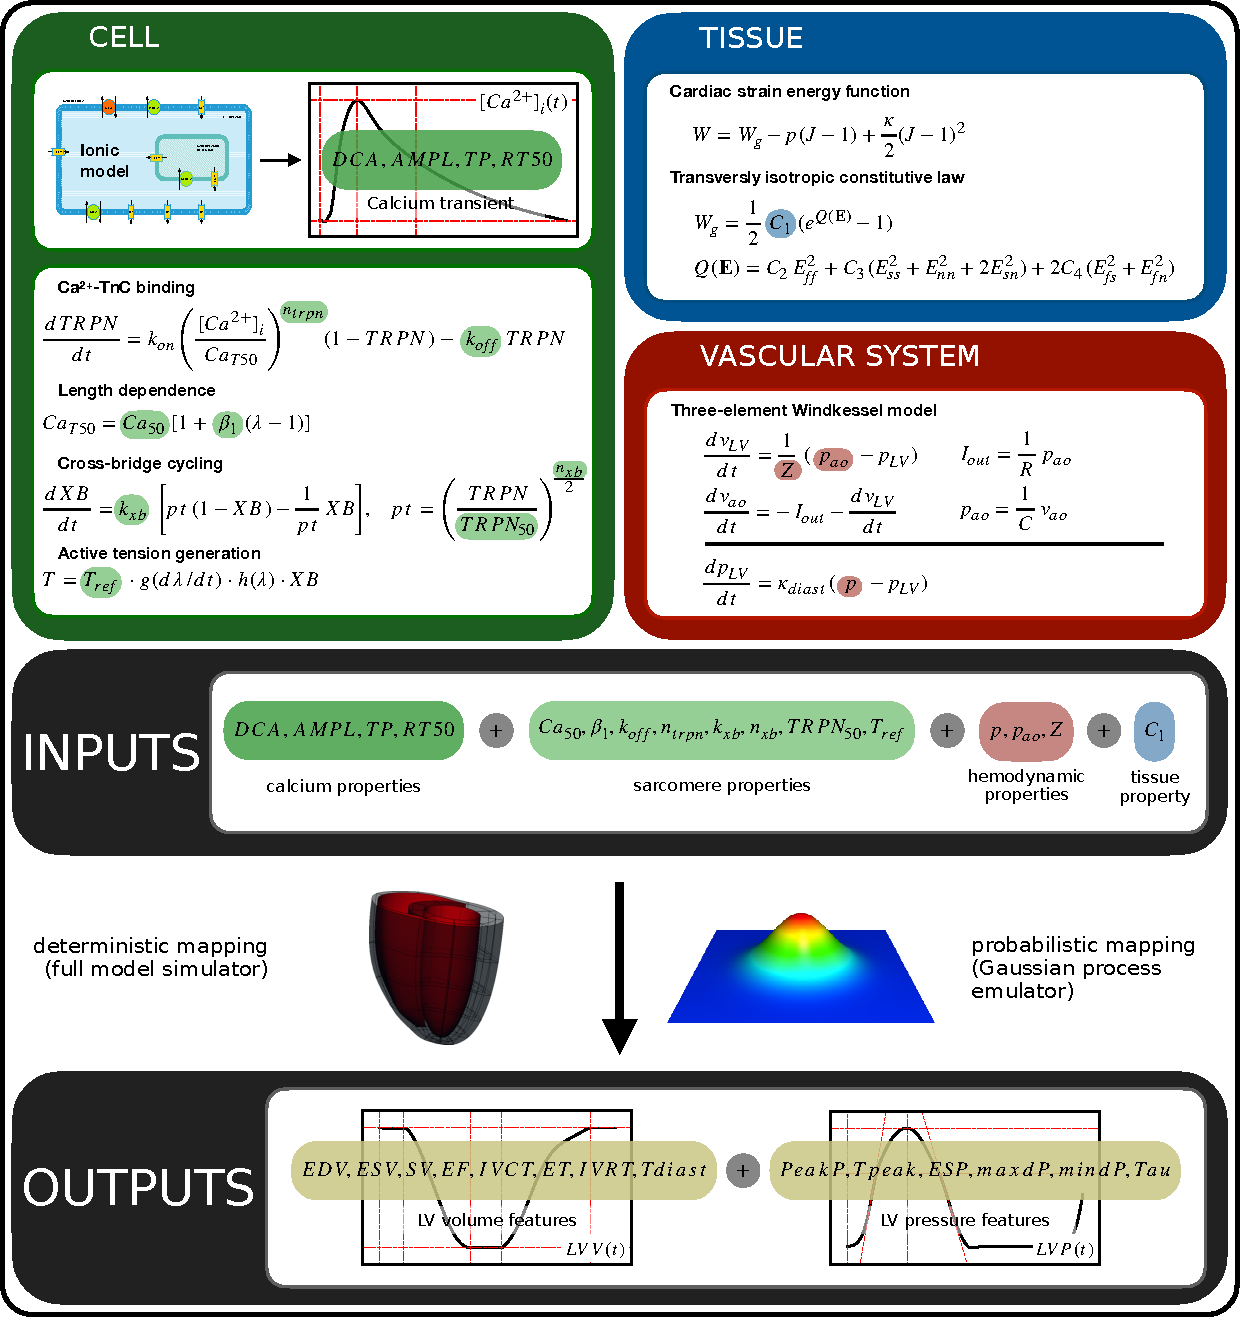
\includegraphics[width=\textwidth]{figures/chapter07/Fig_1.pdf}
    \caption{$\mathbf{3}$D biventricular rat heart contraction model multi-scale map. Chosen $16$ input parameters are calcium transient and sarcomere properties (green), hemodynamics properties (red) and tissue properties (blue). The output features of interest are $14$ indexes (yellow) characterising the LV function and are extracted from the LV pressure and volume curves. The input parameters (Table~\ref{tab:paramswithdeffinal}) can be quantitatively be mapped to the output features (Table~\ref{tab:lvfeaturesfinal}) either by running the full model or by making predictions using trained GPEs.}
    \label{fig:multiscalemap}
\end{figure}


%
%
%
\subsection{Input parameter space}\label{sec:ch7inputparameterspace}
The input parameter space $X\subset\mathbb{R}^{16}$ of the simulator map $f_{simul}$ introduced in equation~\eqref{eq:fsimulfinal} was defined as the hypercube obtained by the Cartesian product of $16$ one-dimensional parameter ranges. Each range was constructed with $\pm$ percentage perturbations of the SHAM model reference parameter values. For the sarcomere, boundary conditions and material properties we varied parameters by $[\SI{50}{\percent},\,\SI{150}{\percent}]$, except for $\beta_1$ which we varied by $[\SI{10}{\percent},\,\SI{200}{\percent}]$. To cover both healthy and pathological calcium transient shapes, we allowed a $[\SI{10}{\percent},\,\SI{200}{\percent}]$ perturbation from reference values for parameters $\dca$, $\ampl$ and $\tp$, while for $\rtf$ the respective scaling coefficient was allowed to induce a $[\SI{10}{\percent},\,\SI{110}{\percent}]$ perturbation. This was done to reject implausible viable curves (Section~\ref{sec:ch6encodingcalciumtransientvariations}). Adopted ranges are reported in Table~\ref{tab:finalparranges}.

\begin{table}[!ht]
    \myfloatalign
    \begin{tabularx}{\textwidth}{XXX}
    \toprule
    \tableheadline{Parameter} & \tableheadline{Units}                   & \tableheadline{Range} \\
    \midrule
    $\dca$                    & $\SI{}{\micro\Molar}$                   & $[0.0463,\,0.9264]$ \\
    $\ampl$                   & $\SI{}{\micro\Molar}$                   & $[0.1034,\,2.0681]$ \\
    $\tp$                     & $\SI{}{\milli\second}$                  & $[2.5947,\,51.8947]$ \\
    $\rtf$                    & $\SI{}{\milli\second}$                  & $[4.0081,\,44.0888]$ \\
    $\Caif$                   & $\SI{}{\micro\Molar}$                   & $[1.0861,\,3.2584]$ \\
    $\betaone$                & $-$                                     & $[-3.00,\,-0.15]$ \\
    $\koff$                   & $\SI{}{\per\milli\second}$              & $[0.0257,\,0.0772]$ \\
    $\ntrpn$                  & $-$                                     & $[1.0,\,3.0]$ \\
    $\kxb$                    & $\SI{}{\per\milli\second}$              & $[0.0086,\,0.0258]$ \\
    $\nxb$                    & $-$                                     & $[2.5,\,7.5]$ \\
    $\trpnf$                  & $-$                                     & $[0.1750,\,0.5250]$ \\
    $\tref$                   & $\SI{}{\kilo\pascal}$                   & $[78.03,\,234.10]$ \\
    $\p$                      & $\SI{}{\kilo\pascal}$                   & $[0.1561,\,0.4683]$ \\
    $\pao$                    & $\SI{}{\kilo\pascal}$                   & $[3.5568,\,10.6704]$ \\
    $\Z$                      & $\SI{}{\mmHg\second\per\milli\liter}$   & $[2.8117,\,8.4351]$ \\
    $\Cone$                   & $\SI{}{kPa}$                            & $[0.4571,\,1.3712]$ \\
    \bottomrule
    \end{tabularx}
    \caption{Input parameters' ranges for the $16$D simulator/emulator.}
    \label{tab:finalparranges}
\end{table}


%
%
%
\subsection{Training dataset, emulators, global sensitivity analysis and history matching}
GP emulation was employed to replace the computationally expensive map from model input parameters to model output LV features. We followed the same emulation framework as in~\cite{Longobardi:2020}. Briefly, we trained the emulators to simulations with parameter values sampled across a $16$-dimensional parameter space.

\vspace{0.2cm}
We sampled $14,848$ points from a LHD over the input parameter space $X$ defined in Section. The simulator was run at these points and the successfully completed simulations were collected to form the training dataset. The final dataset consisted of $1,299$ data points, corresponding to $\SI{8.7}{\percent}$ of the total simulations attempted.

\vspace{0.2cm}
GPEs $f(\mathbf{x})$ were defined as the sum of a

\vspace{0.2cm}
Bayesian history matching (HM) technique was used to re-fit model parameters as done previously~\cite{Longobardi:2020}, to create a mathematical model of the obese ZSF1 rat (Section~\ref{sec:buildingzsf1model}) and to virtually recover it towards an healthy condition (Section~\ref{sec:recovery}).

\vspace{0.2cm}
In order to understand the input parameters impact on the output features total variance we performed a global sensitivity analysis. Model outputs sensitivity to parameters was characterised by Sobol' first-order and total effects~\cite{Kucherenko:2005}. These indexes were estimated using the Saltelli method~\cite{Saltelli:2010} with SaLib Python library~\cite{Herman:2017}. GPErks tool~\cite{Longobardi:2021} was used to incorporate full GPE's posterior distribution samples to account for emulators uncertainty in Sobol' indexes estimates. Parameters whose resulting indexes were below the threshold $0.01$ were determined to have negligible effect.